\documentclass[11pt]{beamer}
\usepackage[T1]{fontenc}
\usepackage[utf8]{inputenc}
\usepackage{lmodern}
\usepackage{tikz}
\usepackage{graphicx}
\usetheme{Madrid}
\usepackage[normalem]{ulem}
\usepackage[absolute,overlay]{textpos}
\usepackage{listings}
\usepackage{courier} 

\setbeamertemplate{navigation symbols}{}
%\setbeamertemplate{footline}[frame number]
\title[Main Title]{Main Title: very very extremely long title}
\subtitle{subtitle}
\author[k4iyer, ssasy, j3tracey]{K. Iyer \and S. Sasy \and J. Tracey}
\institute[]{Cheriton School of Computer Science}
\date{}



\begin{document}

\begin{frame}
  \titlepage
\end{frame}

\begin{frame}{Barrelfish: Overview}
	\begin{itemize}

	\item suitable for scalable operating systems 
		\vfill
	\item multi-cores architecture
		\vfill
	\item heterogeneous architecture
		\vfill
	\item extensions of the seL4 model for distributed capability management between cores
	\end{itemize}
\end{frame}


\begin{frame}{Barrelfish: Capability Types}
\begin{itemize}
\item Main Memory
\vfill
\item Page Tables 
\vfill
\item Device Memory
\vfill
\item Page tables Mapping Memory 
\vfill
\item Kernel interface
\vfill
\item Others
\end{itemize}
\end{frame}


\begin{frame}{Barrelfish: Capability Operations Interaction}
\begin{figure}
		  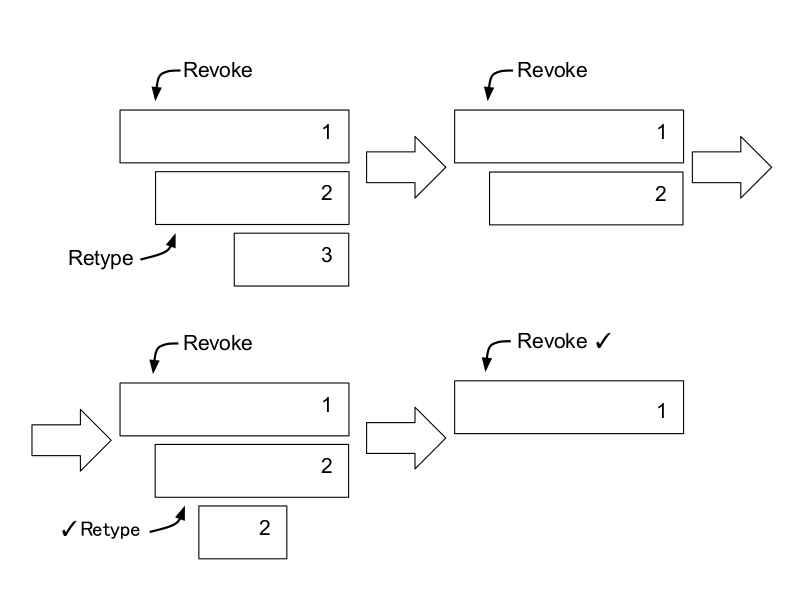
\includegraphics[scale=0.25]{img/BF_revoke_retype}
		  \caption{Revoke-Retype-Delete interactions}
		  
    \end{figure}   
\end{frame}

\begin{frame}{Capsicum: Overview}
	\begin{itemize}
	\item API for implementing capabilities on UNIX
	\vfill 
	\item extends (not replace) standard UNIX APIs by adding kernel-level primitives
	\vfill
	\item new OS primitives for implementing capabilities-
		\begin{itemize}
		    \item capabilities %- refined file descriptors with fine-grained rights
   		    \item capability mode% - process sandboxes that deny access to global namespaces
    		    \item process descriptors% - capability-centric process ID replacement
    		    \item anonymous shared memory objects% - an extension to the POSIX shared memory API to support anonymous swap objects associated with file descriptors (capabilities)
    		    \item rtld-elf-cap% - modified ELF run-time linker to construct sandboxed applications
    		    \item libcapsicum %- library to create and use capabilities and sandboxed components
    		    \item libuserangel %- library allowing sandboxed applications or components to interact with user angels, such as Power Boxes.
    		    \item chromium-capsicum %- a version of Google's Chromium web browser that uses capability mode and capabilities to provide effective sandboxing of high-risk web page rendering.

		\end{itemize}
	\end{itemize}
\end{frame}




\begin{frame}{Capsicum: Example}
	\begin{figure}
		  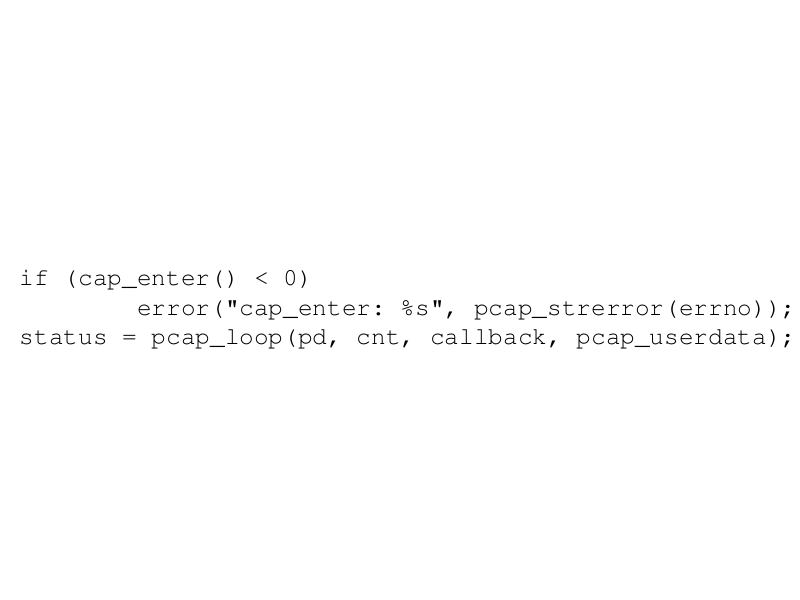
\includegraphics[scale=0.3]{img/tcpdump}
		  \caption{capsicum example}
		  
    \end{figure}  
\end{frame}



\end{document}
